%\documentclass[show notes]{beamer}
%\documentclass[handout]{beamer}
\documentclass[]{beamer}

\usepackage{pgfpages}
\usepackage[utf8]{inputenc}
\usepackage[T1]{fontenc}
%\usepackage{mathabx}
%\usepackage{mathpazo}
%\usepackage{eulervm}
%\usepackage{natbib}
\usepackage{adjustbox}
\usepackage{booktabs}
%\usepackage{svg}
\usepackage{colortbl}
\usepackage{hyperref}
\hypersetup{colorlinks=true, urlcolor=uog, linkcolor=uog, citecolor=uog}

\usepackage[backend=biber, style=authoryear, maxbibnames=99, dashed=false]{biblatex}
\addbibresource{tagged-SWCD2021.bib}


\usepackage{caption}
\captionsetup[figure]{labelformat=empty}% redefines the caption setup of the figures environment in the beamer class.


\usetheme{Madrid}
\definecolor{uog}{rgb}{0,.5,0}
\usecolortheme[named=uog]{structure}

\mode<handout>{
	\pgfpagesuselayout{4 on 1}[letterpaper] 
	\setbeameroption{show notes}
}


% The following code uses \AtBeginSection to place a frame with the section title (\insertsectionhead) inside a beamercolorbox.
% From https://tex.stackexchange.com/questions/178800/creating-sections-each-with-title-pages-in-beamers-slides
\AtBeginSection[]{
	\begin{frame}
		\vfill
		\centering
		\begin{beamercolorbox}[sep=8pt,center,shadow=true,rounded=true]{title}
			\usebeamerfont{title}\insertsectionhead\par%
		\end{beamercolorbox}
		\vfill
	\end{frame}
}

\title[Invasive Species Issues on Guam]{Overview of Invasive Species Issues on Guam}

\author[]{
	Glenn Dulla\textsuperscript{1}, Roland Quitugua\textsuperscript{2} and Aubrey Moore\textsuperscript{2}\\
	\bigskip 
	\tiny{\textsuperscript{1}Guam Department of Agriculture,
    \textsuperscript{2}University of Guam}
}

%\institute[]{College of Natural and Applied Sciences\\University of Guam}

%\titlegraphic{\includegraphics[width=2cm]{big_g2.pdf}}

\date[]{Pacific Ecological Security Conference\\Palau, October 6, 2022\\ \tiny\url{https://github.com/aubreymoore/PESC-OIA-overview/raw/main/guam-overview.pdf}}

\begin{document}
	
%\begin{frame}
    \maketitle
%\end{frame}

\begin{frame}{Hafa Adai}
	\adjincludegraphics[height=1.05\textheight,center]{images/Guam.jpg}
\end{frame}

\begin{frame}{Priority Issues}
	Guam's natural ecosystems, especially Guam's forests, are rapidly being destroyed by invasive species.
	
	
\end{frame}

\begin{frame}{Priority Issue 1: Brown treesnake}
	\adjincludegraphics[height=0.85\textheight,center]{images/bts.jpg}
	\tiny{Courtesy of USGS}
\end{frame}

\begin{frame}{Forest Birds before BTS}
	\begin{figure}
		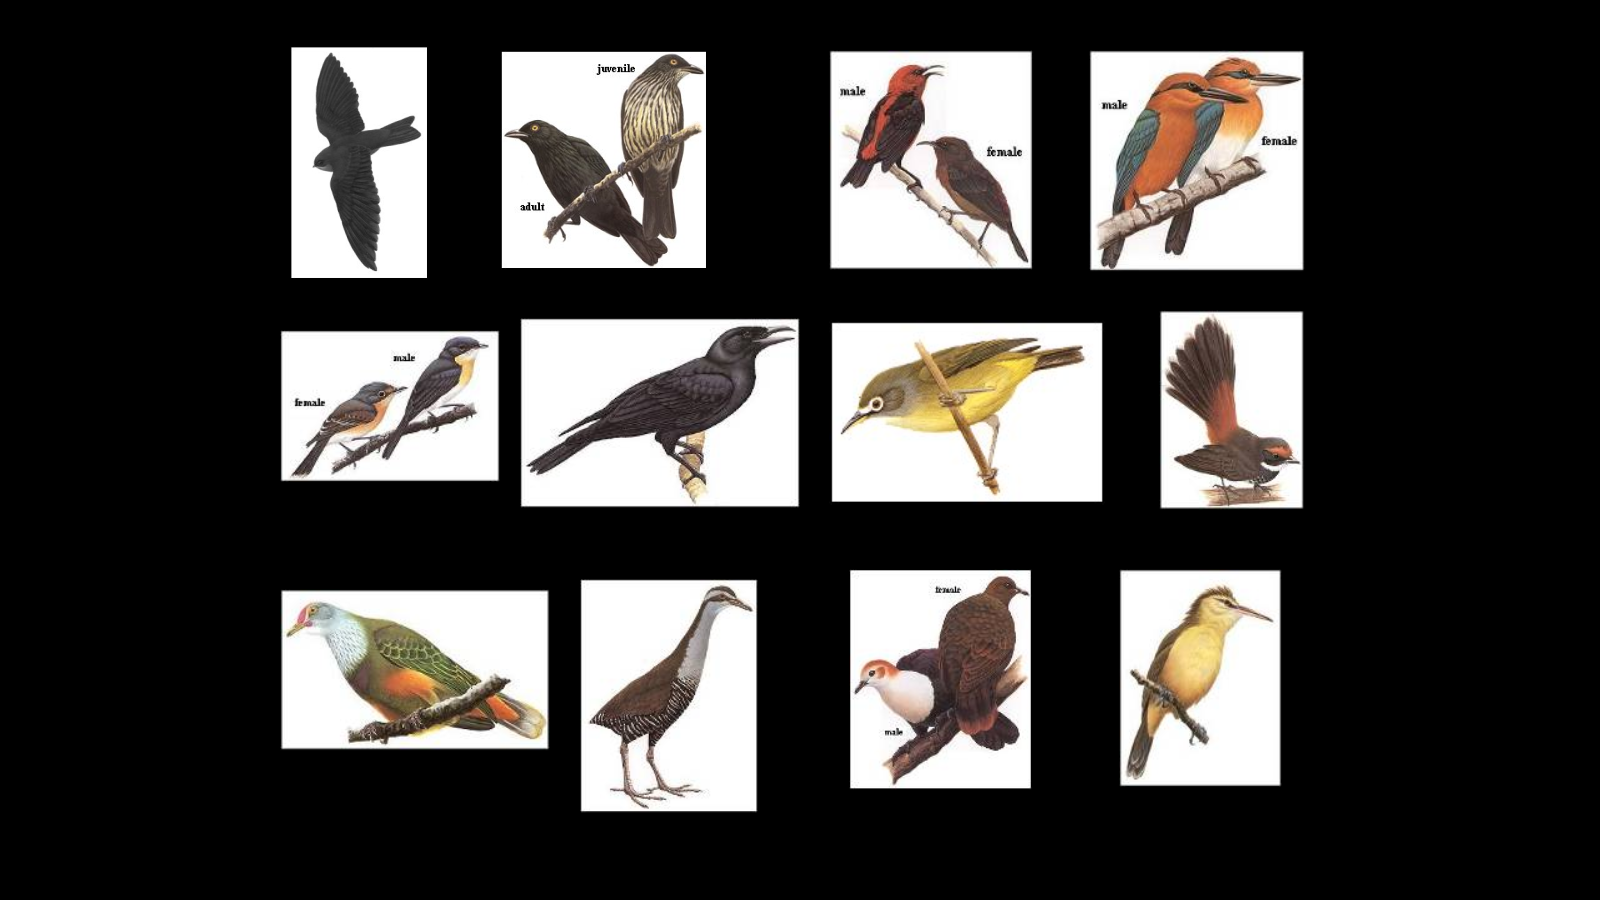
\includegraphics[height=0.8\textheight]{images/birds-before-bts.png}
	\end{figure}
\end{frame}

\begin{frame}{Forest Birds after BTS}
	\begin{figure}
		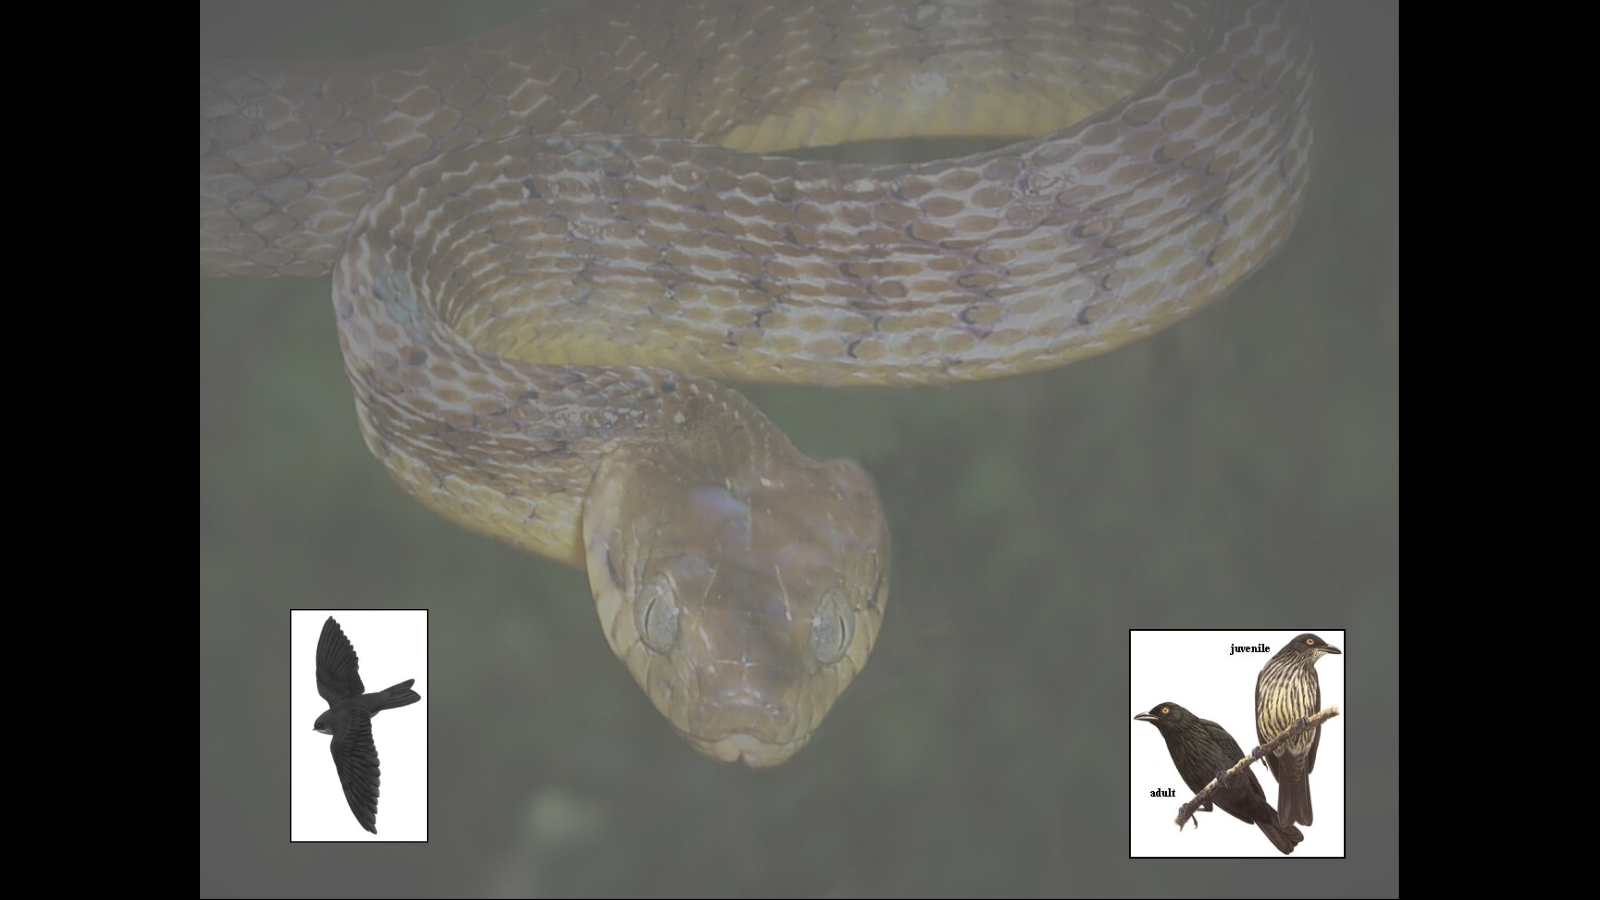
\includegraphics[height=0.8\textheight]{images/birds-after-bts.png}
	\end{figure}
\end{frame}

\begin{frame}{Priority Issue 1: Brown treesnake - Impacts}
	\begin{itemize}
		\item Guam's forest bird species are either extinct or on the endangered species list.
		\item Forest health is severely impacted by the ecosystem services that these birds provided: seed dispersal, insect control, pollination, etc.
	\end{itemize}	
\end{frame}

\begin{frame}{Priority Issue 1: Brown treesnake - Current status}
\begin{itemize}
	\item Established as an invasive species only on Guam since the late 1940s
	\item Millions of dollars per year are spent on preventing BTS from leaving Guam.
	\item Some funds are being used for control methods development: snake-proof barriers and "pinkies on parachutes".
\end{itemize}	
\end{frame}

\begin{frame}{Priority Issue 2: Asian Cycad Scale}
	\adjincludegraphics[width=\textwidth]{images/output-07.png}
\end{frame}

\begin{frame}{Priority Issue 2: Asian Cycad Scale}
	\adjincludegraphics[width=\textwidth]{images/output-19.png}
\end{frame}

\begin{frame}{Priority Issue 2: Cycad aulacaspis scale - Impacts}
	\begin{itemize}
		\item Cycad aulacaspis scale, and other invasive species, have killed about 90\% of Guam's endemic \textit{Cycas micronesica} plants and the population is not recovering because natural reproduction is not occurring.
		\item{\textit{C. micronesica} went from being the most numerous tree in Guam's forests in 2002 to being placed on the National Endangered Species list in 2016}
	\end{itemize}
\end{frame}

\begin{frame}{Priority Issue 2: Cycad aulacaspis scale - Current status}
\begin{itemize}
	\item Established in Hawaii, CNMI, Palau; Cycad population on Yap at great risk.
	\item Cycad aulacaspis scale is partially controlled by introduced predators and parasites on Guam, but almost all seeds and seedlings are being killed by the scale insect.
\end{itemize}	
\end{frame}

\begin{frame}{Priority Issue 3: Coconut rhinoceros beetle}
	\adjincludegraphics[width=\textwidth]{images/outputname-02.png}
\end{frame}

\begin{frame}{Priority Issue 3: Coconut rhinoceros beetle (CRB)}
\end{frame}

\begin{frame}{Priority Issue 4: Little fire ant (LFA)}
		\adjincludegraphics[width=\textwidth]{images/lfa-pencil.jpg}
\end{frame}

\begin{frame}{Challenges}
	\begin{itemize}
		\item Professional scientific/technical capacity is low
		\item Guam suffers from the \textit{taxonomic impediment}
		\item Guam does not have a terrestrial biodiversity inventory
	\end{itemize}
\end{frame}

\begin{frame}{Funding sources}
	\begin{itemize}
	   \item Department of Interior - Office of Insular Affairs
	   \item USDA - Forest Service
	   \item USDA - APHIS
	   \item DOD
	   \item Government of Guam - Invasive Species Tarrif
	\end{itemize}		
\end{frame}

\begin{frame}{National/Territorial Invasive Species Plans}
	\begin{itemize}
		\item Guam Invasive Species Management Plan \url{https://www.sprep.org/attachments/VirLib/Guam/nissap-2017-2019.pdf}
		\item Regional Biosecurity Plan for Micronesia and Hawaii
		\url{https://pacific.navfac.navy.mil/About-Us/Regional-Biosecurity-Plan-for-Micronesia-and-Hawaii/}
	\end{itemize}	
\end{frame}

\begin{frame}{Next steps}
	\begin{itemize}
		\item Implement action items in the Guam Invasive Species Management Plan and the Regional Biosecurity Plan for Micronesia and Hawaii
	\end{itemize}
\end{frame}

\begin{frame}{The End - Thanks for listening.}
	\adjincludegraphics[width=\textwidth]{images/output-53.png}
\end{frame}


\end{document}
